\RequirePackage[l2tabu, orthodox]{nag}		%checks for obsolete LaTeX packages and outdated commands
\documentclass[
	fontsize=11pt,%				Schriftgroesse 11pt
	paper=a4,%					Layout fuer Din A4
	twoside=false,%				Layout fuer beidseitigen Druck %semi %true
	twocolumn=false,%			zweispaltiger Satz
	headsepline=true,%			horizontale Linie unter Kolumnentitel
	footsepline=false,%			Trennline zum Seitenfuß
	headinclude=true,%			Kopfzeile wird Seiten-Layouts mit beruecksichtigt
	footinclude=false,%			Fußzeile wird Seiten-Layouts mit beruecksichtigt
	chapterentrydots=false,%	Inhaltsverzeichnis dotfill für Kapitel
	parskip=false,%				Der erste Absatz eines Abschnitts wird nicht eingezogen
	BCOR=12mm,%					Korrektur fuer die Bindung
	DIV=15,%					DIV-Wert fuer die Erstellung des Satzspiegels, siehe scrguide	%calc
	parskip=half,%				Absatzabstand statt Absatzeinzug
	footnotes=multiple,%		Fußnotenmarkierungen %nomultiple
	headings=openany,%			Kapitel können auf geraden und ungeraden Seiten beginnen %openleft %openright
	index=default,%				Index im Inhaltsverzeichnis %totoc %numbered
	bibliography=totoc,%		Literaturverz. Wird ins Inhaltsverzeichnis eingetragen
	listof=totoc,%				Tabellen und Abbildungs. Wird ins Inhaltsverzeichnis eingetragen
	numbers=noendperiod,%		Kapitelnummern immer ohne Punkt	%endperiod %autoendperiod
	draft=false,%				Keine Bilder in der Anzeige, overfull hboxes werden angezeigt
	titlepage=true,%			Titlei auf erster Seite	%firstiscover
	chapterprefix=false,%		Kapitelprefix für mainmatter
	appendixprefix=true,%		Kapitelprefix für Anhang
	bibliography=oldstyle,%		Formatierungsstil des Literaturverzeichnisses %openstyle
	cleardoublepage=plain,%		Leere seiten plain
	pagesize=auto,%				Ausgabetreiber %pdftex
	]{scrbook}%					crbook 2018/01/23 v3.24

\usepackage{scrhack}
\usepackage{scrwfile}
\usepackage{ifluatex}

\usepackage[english, ngerman]{babel}%		Nötig, damit Dokument in Deutsch generiert wird
\usepackage[utf8]{luainputenc}%				Nötig um Umlaute zu tippen. Alternativ: latin1
\ifluatex
	\usepackage[no-math]{fontspec}
\else
	\usepackage[T1]{fontenc}%				font encoding
\fi

\usepackage[centertags]{amsmath}%	AMS-Mathematik, %centertags zentriert Nummer bei split, %fleqn
\interdisplaylinepenalty=2500
\usepackage{amsthm}
\usepackage{amsfonts}%				Standard fonts
\usepackage{amssymb}%				Standard fonts
\usepackage{gensymb}
\usepackage{array}
\usepackage{mathtools}%				Multiline and split equations
\usepackage{relsize}
\usepackage{physics}

\ifluatex
	\usepackage[luatex]{graphicx}%			Package um grafiken zu includieren
\else
	\usepackage[pdftex]{graphicx}%
\fi
\usepackage{textcomp}%						verschiedene Symbole
\usepackage[onehalfspacing]{setspace}%		Zeilenabstand anpassen
	\KOMAoptions{DIV=last}%					Seitenspiegel durch setspace nicht verändern
\usepackage[hang, bf, font=small, textformat=period]{caption}%	Captions für figures und tables
\usepackage{subcaption}%					Package um subfigure zu erstellen
\usepackage[svgnames, table]{xcolor}%		Farbkonversion etc.
\usepackage{colortbl}%						Support for colors in tables
\usepackage{multirow}%						Zelle einer Tabelle über mehrere Zeilen ausdehnen
\usepackage{booktabs}%						Tabellenformatierung
\usepackage{rotating}%						Rotation von tables und figures
\usepackage{tikz}%							Zeichnen direkt in Latex
\usepackage[siunitx]{circuitikz}%			Zeichnen von elektrischen Schaltbildern direkt in Latex
\usepackage{pgfplots}
	\pgfplotsset{
		compat=newest,%						% TODO: set to current version of pgfplots, when starting your work (2018/01/23: compat=1.15)
		width=0.8\textwidth,%
		colormap={blackwhite}{gray(0cm)=(0); gray(1cm)=(1)},%
	}
\usepackage{siunitx}
	\sisetup{
		locale = DE,%
		detect-all,%
% 		scientific-notation = engineering,%
		list-final-separator = { und },%
		list-pair-separator = { und },%
		range-phrase = { bis },%
		per-mode = symbol,%
		binary-units = true,%
		quotient-mode = fraction,%
		output-complex-root = j,%
	}
	\DeclareSIUnit[]\dBm{dBm}
	\DeclareSIUnit[]\dBW{dBW}
\usepackage{calc}%							Hilfspaket um mit Latex variablen zu rechnen
\usepackage{listings}%						Paket um sourcecode zu publizieren

\lstnewenvironment{matlab}[1][]{
	\lstset{
		backgroundcolor=\color{white}, %\color{TUgreen!20}, %\color{gray!20}
		fillcolor=,% %\color{black},
		captionpos=t,% b
		tabsize=4,%
		rulecolor=\color{black},%
		rulesepcolor=\color{gray!30},%
		language=Matlab,%
		basicstyle=\small,%
		numbers=left,%
		numberfirstline=true,%
		numberblanklines=true,%
		stepnumber=1,%
		numbersep=5pt,%
		numberstyle=\scriptsize,%
		upquote=true,%
		aboveskip={0\baselineskip},%
% 		belowskip=\baselineskip,%
		columns=flexible,% %fixed,
		showstringspaces=false,%
		extendedchars=true,%
		breaklines=true,%
		breakatwhitespace=true,%
		prebreak = \raisebox{0ex}[0ex][0ex]{\ensuremath{\color{black}\hookleftarrow}},%
		breakautoindent=true,%
		frame=single,% %tblr, %shadowbox, %tblrTBLR,
		frameround=ffff,% %tttt,
		showtabs=false,%
		showspaces=false,%
		showstringspaces=false,%
		identifierstyle=\ttfamily,%
		basicstyle=\ttfamily\color{black},%
		keywordstyle=\ttfamily\bfseries\color{MidnightBlue},%
		commentstyle=\color{tudark},% %\color{MediumTurquoise},
		stringstyle=\color{DarkOrchid},%
		mathescape=true,%
		showlines=true,%
		escapechar=§,%							escape to latex
		abovecaptionskip=0\smallskipamount,%
		belowcaptionskip=3\smallskipamount,%
		xleftmargin=1.25\baselineskip,%
		xrightmargin=0pt,
		#1,%									add more options from the optional parameter
	}}{}
\usepackage[
	pdfpagelabels,
	colorlinks=false,
	plainpages=false,
	pdfborder={0 0 0},
	]{hyperref}%						Automatische Kreuzreferenzierungen (auch URLs) im PDF
\makeatletter
\AtBeginDocument{\hypersetup{
		pdftitle = {\@documentnumber},%
		pdfsubject = {\@title},%
		pdfauthor = {\@author},%
		pdfkeywords = {},%
		bookmarksopen = {true},%
		bookmarksdepth = 3,%			up to subsubsection titles will be included into PDF structure
		bookmarksopenlevel = 1,%		... up to section titles
	}
}
\usepackage[acronym,nonumberlist,section=chapter,translate=false,shortcuts,toc=true]{glossaries} % Glossar, Abkürzungsverzeichniss etc.
	\renewcommand{\acronymname}{Abkürzungsverzeichnis}
	\newglossary[slg]{symbol}{sym}{sbl}{Symbolverzeichnis}
	\makeglossaries
	\newglossarystyle{tab_style}{
		\renewenvironment{theglossary}{\begin{longtable}[l]{llp{0mm}}}{\end{longtable}}
		\renewcommand*{\glsgroupheading}[1]{}
		\renewcommand*{\glossentry}[2]{\glsentryitem{##1}\glstarget{##1}{\textbf{\glossentryname{##1}}} & \glossentrydesc{##1} & ##2 \tabularnewline[3px]}
		\renewcommand*{\subglossentry}[3]{\glossentry{##2}{##3}}
		\renewcommand*{\glsgroupskip}{}
	}
	\newglossarystyle{tab_style_sym}{ 
		\renewenvironment{theglossary}{\begin{longtable}[l]{llp{0mm}}}{\end{longtable}}
		\renewcommand*{\glsgroupheading}[1]{}
		\renewcommand*{\glossentry}[2]{\glsentryitem{##1}\glstarget{##1}{\glossentrysymbol{##1}} & \glossentrydesc{##1} & ##2 \tabularnewline[3px]}
		\renewcommand*{\subglossentry}[3]{\glossentry{##2}{##3}}
		\renewcommand*{\glsgroupskip}{}
	}

%%% Symbols
%
\newglossaryentry{pi}{type=symbol,name=\ensuremath{\pi},symbol={\ensuremath{\pi}},sort=pi,description={ratio of circumference of circle to its diameter}}
\newglossaryentry{ohm}{type=symbol,name=ohm,symbol={\ensuremath{\Omega}},description=unit of electrical resistance}
\newglossaryentry{angstrom}{type=symbol,name={\aa}ngström,symbol={\AA},sort=angstrom,description={non-SI unit of length}}
\newglossaryentry{angstro}{type=symbol,name=angstrom,symbol={A},description=non-SI unit of length}


%%% Acronyms

\newacronym{vlc}{VLC}{\textbf{V}isible \textbf{L}ight \textbf{C}ommunication}
\newacronym{david}{DaVid}{\textbf{Da}ta transmission using \textbf{Vi}deo \textbf{d}evices}
\newacronym{surf}{SURF}{\textbf{S}peeded \textbf{U}p \textbf{R}obust \textbf{F}eatures}
\newacronym{sift}{SIFT}{\textbf{S}cale \textbf{I}nvariant \textbf{F}eature \textbf{T}ransform}
\newacronym{ransac}{RANSAC}{\textbf{RAN}dom \textbf{SA}mple \textbf{C}onsensus}
\newacronym{ncc}{NCC}{\textbf{N}ormalized \textbf{C}ross \textbf{C}orrelation}


\newacronym{led}{LED}{\textbf{L}ight-\textbf{E}mitting \textbf{D}iode}
\newacronym{ieee}{IEEE}{\textbf{I}nstitute of \textbf{E}lectrical and \textbf{E}lectronics \textbf{E}ngineers}
\newacronym{abc}{abc}{test}
\newacronym{HDTV}{HDTV}{\textbf{h}igh \textbf{d}efinition \textbf{t}ele\textbf{v}ision}
\newacronym{ISI}{ISI}{inter symbol interference}
\newacronym{gpu}{GPU}{\textbf{G}raphics \textbf{P}rocessing \textbf{U}nit}
\newacronym{eeprom}{EEPROM}{electrically erasable programmable read-only memory}%	load symbol and acronym defintions
\glsaddallunused[\acronymtype]%				add all abbreviations
\glsaddallunused[symbol]%					add all symbols
\makeatother

% *** CITATION PACKAGES ***
\usepackage[style=ieee, backref=false, dashed=false, doi=false, isbn=false, backend=biber]{biblatex}
\usepackage[autostyle=true, german=quotes]{csquotes}
\addbibresource{literatur.bib}

\DeclareBibliographyDriver{standard}{%
	\usebibmacro{bibindex}%
	\usebibmacro{begentry}%
	\usebibmacro{author/editor+others/translator+others}%
	\setunit{\labelnamepunct}\newblock
	\usebibmacro{maintitle+title}%
	\newunit\newblock
	\printfield{version}%
	\newunit\newblock
	\printfield{series}%
	\newunit\newblock
	\printfield{number}%
	\iffieldundef{number}{%
		\newunit\newblock
		\printfield{type}%
	}{%
		\setunit{\addspace}\newblock
		\printfield[parens]{type}%
	}
	\newunit\newblock
	\printfield{note}%
	\newunit\newblock
	\usebibmacro{organization+location+date}%
	\newunit\newblock 
	\usebibmacro{chapter+pages}% 
	\newunit 
	\printfield{pagetotal}% 
	\newunit\newblock
	\iftoggle{bbx:isbn}
		{\printfield{isbn}}
		{}%
	\newunit\newblock
	\iftoggle{bbx:url}
		{\usebibmacro{url+urldate}}
		{}%
	\newunit\newblock 
	\usebibmacro{addendum+pubstate}%
	\setunit{\bibpagerefpunct}\newblock
	\usebibmacro{pageref}%
	\newunit\newblock
	\usebibmacro{related}%
	\usebibmacro{finentry}}

\usepackage[german]{cleveref}

% WASSERZEICHEN
% \usepackage{draftwatermark}
% \SetWatermarkText{Draft}
% \SetWatermarkLightness{0.9}
% \SetWatermarkScale{1}

% Schrift
\ifluatex
	% Arial
	\setmainfont{Arial}
	\setsansfont{Arial}
	% or Calibri
% 	\setmainfont{Calibri}
% 	\setsansfont{Calibri}
	\usepackage[italic]{mathastext}
\else
	\usepackage{helvet}
	\renewcommand{\familydefault}{\sfdefault}
	\usepackage[helvet]{sfmath}
	\usepackage{sansmathaccent}
\fi

% TU Farben
\xdefinecolor{tugreen}{RGB}{132, 184, 24}%		0
\colorlet{tulight}{tugreen!20!white}%			1
\colorlet{tudark}{tugreen!60!black}%			2
\xdefinecolor{tuorange}{RGB}{227, 105, 19}%		3
\xdefinecolor{tuyellow}{RGB}{242, 189, 0}%		4
\xdefinecolor{tucitron}{RGB}{249, 219, 0}%		5

% Nummerierung in den Überschriften bis Ebene...
% \setcounter{secnumdepth}{4}
% \setcounter{tocdepth}{4}

% Fußnoten mit Buchstaben
% \renewcommand{\thefootnote}{\alph{footnote}}

% Verzeichnisnamen
% \renewcommand{\contentsname}{}
% \renewcommand{\listfigurename}{}
% \renewcommand{\listtablename}{}
% \renewcommand{\refname}{}
% \renewcommand{\abstractname}{}
\renewcommand*{\lstlistingname}{Quellcode} % Listings umbenennen
\renewcommand{\lstlistlistingname}{Quellcodeverzeichnis} % Listingsverzeichnis umbenennen

% Todo environment
\newenvironment{TODO}[1]{\textcolor{red}{\textbf{TODO: #1}}}

% Bilder
\graphicspath{./images/}
\DeclareGraphicsExtensions{.pdf,.png,.jpg}

% Titelei
\usepackage{kt_title}
\usepackage{lipsum}	% TODO: remove. This is for dummy text only

%%%%%%%%%%%%%%%%%%%%%%%%%%%%%%%%%%%%%%%%%%%%%%%%%%%%%%%%%%%%%%%

\thesistitle{Tasty Kanalmodell\\ für die drahtlose Kommunikation\\ zwischen Gebäuden und\\ Außeninstallationen} % Titel der Abschlussarbeit % no more than 4 lines here
\documentnumber{B\ 14-2015}%	MXX-20XX
\documenttype{Bachelorarbeit}%	Masterarbeit
\authorfirstname{Käpt'n Kevin}%	Name des Autors
\authorsurname{Blaubär}%		Nachname des Autors
\matrikelnumber{123456}%		Matrikelnummer des Autors
\date{23. Januar 2018}%			Abgabedatum

\makeatletter
\title{\@thesistitle}
\author{\@authorfirstname\space\@authorsurname}
\makeatother

%%%%%%%%%%%%%%%%%%%%%%%%%%%%%%%%%%%%%%%%%%%%%%%%%%%%%%%%%%%%%%%

\begin{document}
\frontmatter
\pagestyle{empty}
\maketitle
% \include{frontmatter/acknoledgement}
\pagestyle{headings}
% \include{frontmatter/abstract}
\tableofcontents%			Inhaltsverzeichnis

\mainmatter
\chapter{Einleitung} \label{cha:Einleitung}

In den letzten Jahren hat \gls{vlc} sowohl in der Wissenschaft als auch in der Industrie große Aufmerksamkeit erregt. Aufgrund seiner Vorteile hinsichtlich Bandbreitenverfügbarkeit, Sicherheit und Datensicherheit wird \gls{vlc} in vielen Anwendungen als eine bessere Alternative zur Radiofrequenz und Infrarot betrachtet, wie z.B. drahtloses Netzwerk mit Beleuchtungssystem\cite{1205458}, Innenraumpositionierung \cite{4649677}, optische Verbindungen zu elektronischen Chips \cite{867694}, Körpersensornetzwerken \cite{bodysensor}, usw. Viele dieser \gls{vlc}-Techniken wurden entwickelt, um bereits vorhandene Lichterzeugungsgeräte zu nutzen. Ein innovativer Ansatz ist die Verwendung von Display-Kamera-Paaren zur Datenübertragung. Aufgrund der steigenden Performance der beteiligten Schlüsselkomponenten erscheinen Datenraten von bis zu 100 Mbit/s realisierbar, während gleichzeitig eine Videopräsentation für menschliche Zuschauer auf dem gleichen Bildschirm zur Verfügung gestellt werden kann. Mit einem solchen System können viele innovative Medienanwendungen realisiert werden.

\section{Motivation} 

In einer aktuellen Forschung untersucht der Lehrstuhl für Kommunikationstechnik an der TU Dortmund ein neuartiges Verfahren der Visible Light Communication: Das \gls{david}-System, welches eine optische Freiraum-Übertragung unter Verwendung verfügbarer Displays und Kameras durchführt. Ein Highlight dieses Systems ist, dass sie die ursprüngliche Funktionalität des Displays nicht beeinträchtigt; Während der Datenübertragung kann das Display immer noch statische Bilder oder Videos anzeigen, ohne dass menschliche Betrachter die versteckten Datensignale wahrnehmen. Die Übertragungsdaten werden in einem Videosignal in Form geringer Amplitudenänderungen differentiell überlagert. Am Empfänger lässt sich der Display durch eine Kamera oder Smartphone optische aufnehmen. Anschließend können die überlagerte Daten empfangen und decodiert werden. Hierzu ist es notwendig, den Modulationsbereich, der durch die optische Projektion verzerrt wird, mit einigen Operationen wiederherzustellen.

\section{Aufgabe in dieser Arbeit} 

In dieser Arbeit werden zwei Verfahren zur Ausschnittsdetektion für Differenzbilder untersucht und implementiert. Die erste Methode verwendet die Charakteristiken der Datenmodulation des \gls{david} Systems, d.h. auf dem Differenzbild wird das QR Muster detektiert, um den Modulationsbereich zu bestimmen. Das zweite Verfahren basiert auf der Geometrie des Displays. Mit Verwendung der Radon Transformation kann der rechteckige Modulationsbereich bestimmt werden. Darüber hinaus wird in dieser Arbeit ein Modul zu Bilderkennung entwickelt, welches die Videostabilität bei Aufnahme mit dem Smartphone aus der Hand verbessern kann. Außerdem durch Einführung des Begriffs der $ ``Energie" $ wurde eine Optimierungsmethode für Differenzbilder entwickelt. Im Anschluss wurde die Performance der beiden Verfahren evaluiert. Das zweite Verfahren wurde auf einer Smartphone-GPU implementiert.

\section{Aufbau der Arbeit} 

Der Rest des Dokuments ist wie folgt organisiert. Das nachfolgende Kapitel gibt eine Beschreibung über das \gls{david} System. Es stellt die Struktur und Arbeitsweise des \gls{david} Systems vor und listet verschiedene Anwendungsbereiche auf, die möglicherweise vom \gls{david}-Konzept profitieren könnten. Der dritte und vierte Absatz enthält Informationen zu beiden Verfahren. Die Struktur und Zusammensetzung der Methoden werden vorgestellt und das Arbeitsprinzip jedes Teils wird detailliert beschreibt. Das nächste, also fünfte Kapitel, zeigt die Implementierung jeder Methode. Darin können die Wirkung jedes Teils in der Methode gesehen werden. %Schließlich zeigt die Implementierung auf eine Smartphone-GPU.
Kapitel 6 enthält eine Evaluierung der beiden Verfahren. Die Performance des Verfahrens werden analysiert. Der letzte Abschnitt schließt die Ergebnisse ab und gibt einen Ausblick auf die zukünftige Arbeit.
\chapter{Grundlagen} \label{cha:Grundlagen}

Nicht vergessen, dass Überschriften nicht aufeinander folgen dürfen\ldots


\section{Section} \label{sec:Section2}

Label Beispiel (vgl. \cref{sec:Section})

% a example citation
\cite{Kammeyer}

% using glossary entries. symbols and acronyms are defined in backmatter/symbols_and_acronyms
\gls{ieee}

\gls{ieee}

\gls{abc}

\gls{led}

\glssymbol{angstrom} \gls{angstrom}

\gls{led}

% example equation
The ratio of the circumference of a circle to its diameter is given by \gls{pi}:
\begin{equation}
\glssymbol{pi} = \frac{C}{d} \cdot \glssymbol{ohm}
\end{equation}

\begin{equation}
U = R \cdot I
\end{equation}


% example figure
\begin{figure}[htbp]
\centering
\begin{circuitikz}[european inductors, european resistors]
\draw [help lines] (0,0) grid (8,4);
\draw
(0,0) node[anchor=east]{} to [short, o-](8,0)
(0,4) node[anchor=east]{} to [short,i=$\textbf{i}_s^s$, o-](1,4)
to[R,l=$\text{R}_{\text{s}}$](3,4)
to[L,l=$\text{L}_{\text{sl}}$](5,4)
to[L,l=$\text{L}_{\text{rl}}$,i>=$\textbf{i}_r^s$](8,4)
to[R,l=${\text{R}'}_{\text{r}}$](8,2) -- (8,1.5) (8,1) -- (8,0) (5,4)
to[L,i>^=$\textbf{i}_m^s$,l=$\text{L}_{\text{m}}$,-*](5,0)
;\draw
(8,1) node[fill=white,shape=circle,minimum size=30,draw,
label={[xshift=0.5cm, yshift=-0.2cm]\textbf{+}},
label={[xshift=1.2cm, yshift=-0.8cm]j$\omega_r\mathbf{\varPsi}_r^s$}]{}
;
\end{circuitikz}
\captionbelow{Dynamic equivalent circuit for an induction machine}
\label{fig:dyneqmodel}
\end{figure}

% some siunitx examples

\num{12345,67890} \\
\num{1+-2i} \\
\num{.3e45} \\
\num{1.654 x 2.34 x 3.430}

\si{kg.m.s^{-1}} \\
\si{\kilogram\metre\per\second} \\
\si[per-mode=symbol]
{\kilogram\metre\per\second} \\
\si[per-mode=symbol]
{\kilogram\metre\per\ampere\per\second}

\numlist{10;20;30}
\SIlist{0.13;0.67;0.80}{\milli\metre} \\
\numrange{10}{20} \\
\SIrange{0.13}{0.67}{\milli\metre}

\newglossaryentry{c0}{type=symbol,name=c0,symbol={\si{\clight}},description={\SI[scientific-notation = engineering]{299792458}{\meter\per\second}, speed of light}}

\glssymbol{c0}
\newpage
\section{Hello newpage}

\begin{table}[htb]
\centering
\captionabove{Dies ist nur eine Beispieltabelle}
\label{tbl:beispiel}
\begin{tabular}{l|lll}
Dies & ist & ein & Beispiel.\\\hline
Bitte & lassen & Sie & den \\
Inhalt & dieser & Tabelle & unbeachtet.
\end{tabular}
\end{table}

Booktabs Tabellenbeispiel

\begin{table}[htb]
	\captionabove[IEEE~802.11a und IEEE~802.11p PHY-Parameter im Vergleich]{IEEE~802.11a und IEEE~802.11p PHY-Parameter im Vergleich\,\cite{IEEE2012}}
	\label{tbl:params}
	\footnotesize
	\centering
	\rowcolors{2}{white}{gray!25}	%TUgreen!25
	\begin{tabular}{m{5cm}*{2}{c}}	%p{}m{}b{}clr
	\toprule
	\textbf{Parameter} & \textbf{IEEE~802.11a} & \textbf{IEEE~802.11p} \\
	\midrule
	Kanalbandbreite $B$ & \SI{20}{\mega\hertz} & \SI{10}{\mega\hertz} \\
	Maximale Sendeleistung $P_\text{S}$ & \SI{20}{\dBm} & \SI{33}{\dBm} \\
	Datenrate [\si{\mega\bit\per\second}] & 6, 9, 12, 18, 24, 36, 48, 54 & 3, 4.5, 6, 9, 12, 18, 24, 27 \\
	Modulationen & BPSK, QPSK, 16-QAM, 64-QAM & BPSK, QPSK, 16-QAM, 64-QAM \\
	Coderaten & \num{1 / 2}, \num{2 / 3}, \num{3 / 4} & \num{1 / 2}, \num{2 / 3}, \num{3 / 4} \\
	Anzahl Datensubträger ($N_{\text{SD}}$) & 48 & 48 \\
	Anzahl Pilotsubträger ($N_{\text{SP}}$) & 4 & 4 \\
	Gesamtanzahl Subträger ($N_{\text{ST}}$) & 52 ($N_{\text{SD}} + N_{\text{SP}}$) & 52 ($N_{\text{SD}} + N_{\text{SP}}$) \\
	Subträgerabstand ($\Delta f$) & \SI{312.50}{\kilo\hertz} ($\frac{\SI{20}{\mega\hertz}}{\num{64}}$) & \SI{156.25}{\kilo\hertz} ($\frac{\SI{10}{\mega\hertz}}{\num{64}}$) \\
	Dauer (Inverse) Fast Fourier\-trans\-for\-ma\-tion ($T_{\text{FFT}}$) & \SI{3.2}{\micro\s} ($\frac{1}{\Delta f}$) & \SI{6.4}{\micro\s} ($\frac{1}{\Delta f}$)\\
	Dauer Guard Interval $T_{\text{GI}}$ & \SI{0.8}{\micro\s} ($\frac{T_{\text{FFT}}}{4}$) & \SI{1.6}{\micro\s} ($\frac{T_{\text{FFT}}}{4}$) \\
	Dauer Training Symbol GI $T_{\text{GI2}}$ & \SI{1.6}{\micro\s} ($\frac{T_{\text{FFT}}}{2}$) & \SI{3.2}{\micro\s} ($\frac{T_{\text{FFT}}}{2}$) \\
	Symbol Interval $T_{\text{SYM}}$ & \SI{4}{\micro\s} ($T_{\text{GI}} + T_{\text{FFT}}$) & \SI{8}{\micro\s} ($T_{\text{GI}} + T_{\text{FFT}}$) \\
	Präambellänge $T_{\text{Preamble}}$ & \SI{16}{\micro\s} & \SI{32}{\micro\s} \\
	\bottomrule
	\end{tabular}
\end{table}

Quellcodebeispiel mit Seitenumbruch

\singlespacing
\begin{matlab}[firstnumber=1, name=MATLABCodeBeispiel, caption={MATLAB Code Beispiel}, label={lst:MATLABCodeBeispiel}]
%instrreset
clear all
oldobjs=instrfind;
if ~isempty(oldobjs)
disp('Cleaning up ...')
delete(oldobjs);
clear oldobjs;
end

close all;
clear all;


samprate = 65833332;    % 65833333 disables HF Filter  % Sample Rate
trigger = 'IMM';        % Trigger setting. IMM, IFP or EXT
nosamples = 8000;       % No. Captured IQ Sample Pairs. Max 2 MB also 262144 IQ/Samples
dispupdate = 'On';      % Analyser Display On or Off

freq_center = 2412e6;
channel_bw = 20e6;
power_level = -40; % [dBm]
\end{matlab}
\onehalfspacing

\begin{figure}[htbp]
	\centering
	\begin{tikzpicture}
		\begin{axis}[
		title={$x \exp(-x^2-y^2)$},
		xlabel=$x$, ylabel=$y$,
		]
		\addplot3[
		surf,				%contour gnuplot		% for gnuplot test
		domain=-2:2,
		domain y=-1.3:1.3,
		]
		{exp(-x^2-y^2)*x};
		\end{axis}
	\end{tikzpicture}
	\captionbelow{Plot of a Math Expression}
	\label{fig:mathplot}
\end{figure}
\chapter{Implementierung} \label{cha:Implementierung}

Nicht vergessen, dass Überschriften nicht aufeinander folgen dürfen\ldots

\begin{otherlanguage}{english}
\section{TexLipse spell checking}
%
To enable spell checking in TeXLipse, download the respective dictionaries from 
\url{https://sourceforge.net/projects/texlipse/files/dictionaries/}.

Save the dictionaries at a local location and enter the path in \texttt{Window->Preferences->Tex\-lipse->Spell Checker} (see Fig. \ref{fig:dict_path}).
%
\begin{figure}[htb]
	\centering
	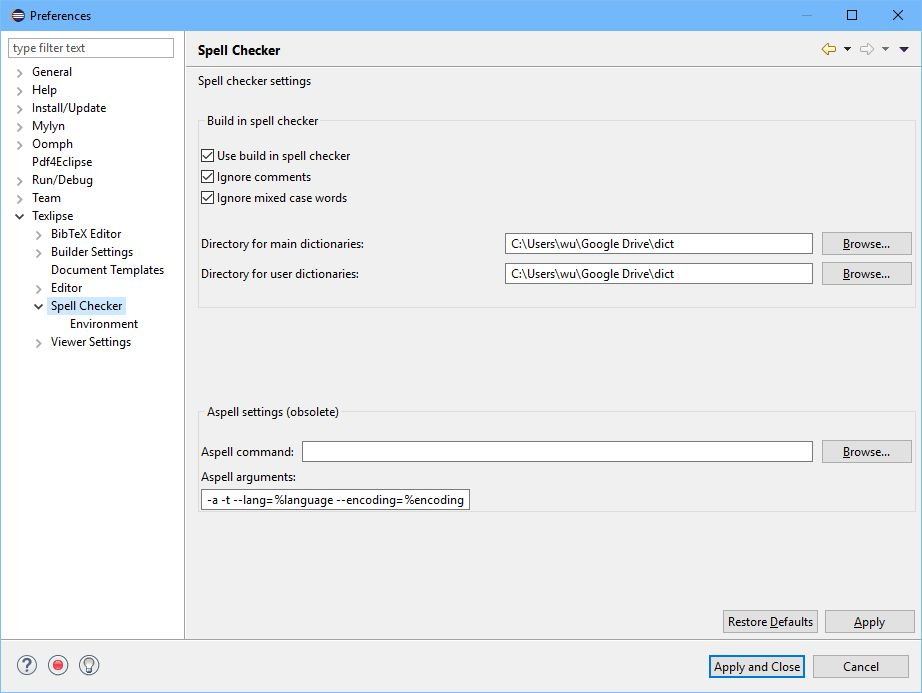
\includegraphics[scale=0.40]{images/Spell_Checker_preferences.jpg}
	\captionbelow{TeXLipse Spell Checker preferences}
	\label{fig:dict_path}
\end{figure}

To synchronize the user dictionaries between multiple machines, it might be useful to save the dictionaries in your google drive or drop box.

\section{Enable tikzexternalize for PdfLatex}

Go to \texttt{Window->Preferences->Texlipse->Builder Settings} and add 
%
\begin{verbatim}
--shell-escape
\end{verbatim}
%
to the command arguments (see Fig. \ref{fig:builder_settings}).
%
\begin{figure}[htb]
	\centering
	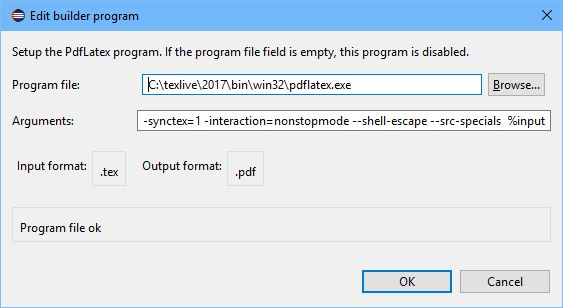
\includegraphics[scale=0.40]{images/PdfLatex_settings.jpg}
	\captionbelow{PdfLatex Builder Settings}
	\label{fig:builder_settings}
\end{figure}

\section{Forward search with TeXlipse and Sumatra PDF}

Download and install SumatraPDF: \url{https://www.sumatrapdfreader.org/}.

Then edit the viewer settings for SumatraPDF in \texttt{Window->Preferences->Texlipse->Viewer Settings}.

Change the viewer arguments to
%
\begin{verbatim}
-reuse-instance %fullfile -forward-search %texfile %line
\end{verbatim}
%
and leave all DDE message field empty.
Change the inverse search support to "`Viewer runs external command"' and enable "`Viewer supports forward search"'.

Figure \ref{fig:viewer_settings} displays the dialog window.
%
\begin{figure}[htb]
	\centering
	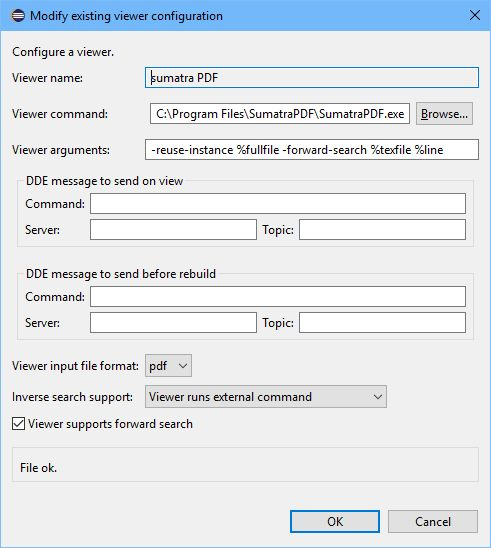
\includegraphics[scale=0.40]{images/Viewer_settings.jpg}
	\captionbelow{TeXLipse Viewer Settings}
	\label{fig:viewer_settings}
\end{figure}

In SumatraPDF configure the inverse search command via the \texttt{Settings->Options} menu (see Fig. \ref{fig:sumatrapdf_options}).
%
\begin{figure}[htb]
	\centering
	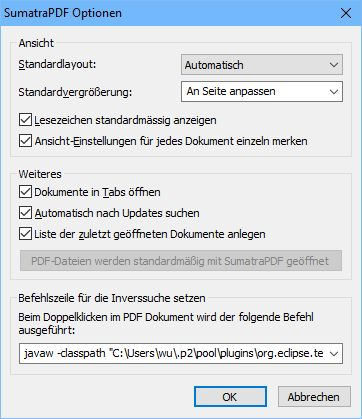
\includegraphics[scale=0.40]{images/SumatraPDF_optionen.jpg}
	\captionbelow{SumatraPDF Options}
	\label{fig:sumatrapdf_options}
\end{figure}

If you have install TeXlipse~1.5.0, the inverse search command will look like this:

\begin{lstlisting}[breaklines=true, basicstyle=\ttfamily, columns=flexible]
javaw -classpath "C:\Users\wu\.p2\pool\plugins\net.sourceforge.texlipse_1.5.0\texlipse.jar" net.sourceforge.texlipse.viewer.util.FileLocationClient -p 55000 -f "%f" -l %l
\end{lstlisting}

Let the path point to your eclipse share pool. Or if you do not have a shared pool, choose the plugins directory of your eclipse installation.

For TeXLipse~2.0.X the FileLocationClient is relocated to org.eclipse.texlipse making the inverse search command look like the following.
\begin{lstlisting}[breaklines=true, basicstyle=\ttfamily, columns=flexible]
javaw -classpath "C:\Users\wu\.p2\pool\plugins\org.eclipse.texlipse_2.0.1.201801202105\texlipse.jar" org.eclipse.texlipse.viewer.util.FileLocationClient -p 55000 -f "%f" -l %l
\end{lstlisting}

\end{otherlanguage}
\chapter{Auswertung} \label{cha:Auswertung}

Text hier zwischen. Referenz auf ein Bild mit cleverref (siehe \cref{fig:mathplot}). Und dann noch ein paar Zitierungen \cite{Reinhold:2013fk,Moon,IEEE2011}.

\section{Section}

Jetzt nur noch schreiben! :)



\chapter{Zusammenfassung} \label{cha:Zusammenfassung}

In dieser Arbeit werden zwei Verfahren zur Ausschnittsdetektion für die Screen-Camera Visible Light Communication untersucht und implementiert. Methode 1 ist vom differentiellen Modulationsverfahren des David-Systems inspiriert. d.h. Daten werden mit geringer Amplitude im Videosignal differentiell überlagert. In der Methode wird ein QR Muster an jeder Ecke der Datenebene hinzugefügt und dann mit den Daten zusammen hinter dem Bild moduliert. Diese Methode kann nicht nur den unschönen Effekt lösen, welcher durch direktes Hinzufügen des QR Musters zu dem Videobild verursacht wird, sondern kann auch den QR Muster durch seine spezifische geometrische Eigenschaft, d.h. in jeder Richtung beträgt das Breiteverhältnis $1:1:3:1:1$, effektiv erkennen. Dadurch wird schließlich der Modulationsbereich bestimmt. Das 2. Verfahren wird in den physikalischen Eigenschaften des Modulationsbereichs ausgeführt. Im \gls{david} System wirkt der Bildschirm als Übertragungsende, und der Bildschirmbereich ist der Modulationsbereich, der im Allgemeinen in Form eines Rechtecks ist. Dadurch kann dieses Problem in eine rechteckige Erkennung umgewandelt werden. Durch die Radon Transformation wird die längste gerade Linie in dem Bild detektiert, um ein Rechteck bzw. den Modulationsbereich, zu bestimmen.

zwei Aufnahmebedingungen wurden in dieser Arbeit berücksichtigt, eine ist die Aufnahme mit dem Smartphone aus der Hand und die andere auf einem Stativ. Handheld-Kamera-Shooting ist eine der häufigsten und bequemsten Aufnahmemethoden im Alltag, und hat eine unerlässliche Position in der praktischen Anwendung. Zu diesem Zweck wurde ein Bildregistrierungsmodul speziell für Handschütteln entwickelt, welche Merkmals Detektion, \gls{ransac}, Kamera Modell und Nichtlineare Optimierung beinhaltet. Beim Testen beträgt die relative Verschiebung zwischen den entsprechenden Punkten des korrigierten Bildes c.a. 0.3 Pixel. Dies führt zu einem relativ guten Differenzbild. Dieser spielte eine wichtige Rolle weil beide Verfahren in dieser Arbeit auf der Detektion von Differenzbildern basieren. Dafür wird der Begriff $ ``Energie" $ eingeführt, welcher die Klarheit des Modulationsbereichs repräsentiert. Gemäß der Energiesortierung werden die klarsten Bilder ausgewählt und hinzugefügt, um das zu detektierende Bild zu erhalten. In Methode 1 werden die beide obigen Schritte implementiert, und durch Auswertung die durchschnittliche Abweichung ca. $ 1-2 $ Pixel bemessen. Es sollte hier angemerkt werden, dass aufgrund der Eigenschaften der Bildregistrierung das Video, das in Methode 1 aufgenommen wurde, ein statisches Video ist, d.h. der Inhalt des Videos hat sich nicht geändert. Der Grund dafür ist, dass der Punkt der Merkmals Detektion hauptsächlich auf dem Inhalt des Videos basiert. Wenn sich der Videoinhalt stark ändert, ist es schwierig, die Genauigkeit der Bildwiederherstellung zu garantieren. Einige bei der Arbeit versuchten Methoden war die Abschirmung des zentralen Bereichs während der Merkmals Detektion, d.h. nur die Merkmale in der Umgebung des Bildes wurden erkannt, was nicht zufriedenstellend ist. Methode 2 implementiert die Erkennung des Modulationsbereichs unter Verwendung eines Stativs. Nach der Erkennung beträgt die durchschnittliche Abweichung ebenfalls ca. $ 1-2 $ Pixel. In beiden Methoden kann der Modulationsbereich mit Parametern, wie die Modulationsapmlitude als 4,  der Datenblock als $ 4 \times 4 Pixel$, erfolgreich bestimmt werden. 

Für dieses Thema gibt es einige mögliche weitere Forschung in der Zukunft. Zuerst kann wie oben erwähnt, ein Verfahren gefunden werden, welches beim Aufnehmen des dynamischen Videos mit dem Smartphone aus der Hand, das Handschütteln-Problem effektiv löst. Der Fokus liegt darauf, die Wirkung vom Video-Inhalt zu neutralisieren und das Bild nur auf die Merkmale des Hintergrunds zu filtern. Zweitens, die in dieser Arbeit verwendete Differenzbild Optimierungsmethode, kann aufgrund der Berechnung der $ ``Energie" $ für jedes Differenzbild zu einer großen Rechenlast führen. Ein effektives Verfahren wäre versuchen, ein zu detektierendes Bild, das auf dem bekannten Differenzbild basiert, effizient zu generieren. Schließlich wurde in Experiment festgestellt, dass unter denselben Parametern die Verwendung des gleichen Smartphones mit dem gleichen Video-Inhalt auf verschiedenen Bildschirmen, zu unterschiedlichen Ergebnissen führt. Dadurch können die Auswirkungen der Bildschirmfaktoren, wie z.B. Beleuchtungsart, Auflösung, Bildwiederholfrequenz, weiter erforscht werden.






\appendix
\chapter{Erster Anhang} \label{cha:anhangA}

\section{Section}

Jetzt nur noch schreiben! :)




\backmatter
\cleardoublepage
% \chapter*{Nomenklatur} \addcontentsline{toc}{chapter}{Nomenklatur}
% \markboth{Nomenklatur}{Nomenklatur}

\printglossary[type=\acronymtype, style=tab_style] %[toctitle=Symbolverzeichnis,title=Symbolverzeichnis] 
\printglossary[type=symbol, style=tab_style_sym]
% \printglossary

\listoffigures%				Abbildungsverzeichnis
\listoftables%				Tabellenverzeichnis
\lstlistoflistings%			Listingsverzeichnis

% \nocite{*}%				es wird alles zitiert
\printbibliography%			Literaturverzeichnis

\makeatletter
\cleardoublepage
\thispagestyle{empty}
\onehalfspacing
\LARGE
\begin{center}
	\textbf{Eidesstattliche Versicherung}
\end{center}

\small
\vspace{\baselineskip}
\underline{\makebox[.4\textwidth][c]{\@authorsurname,\space\@authorfirstname}}
\hspace{.25\textwidth}
\underline{\makebox[.3\textwidth][c]{\@matrikelnumber}}
\newline
\makebox[.4\textwidth][l]{Name, Vorname}
\hspace{.25\textwidth}
\makebox[.3\textwidth][l]{Matr.-Nr.}

Ich versichere hiermit an Eides statt, dass ich die vorliegende \@documenttype\space mit dem Titel

\underline{\makebox[0.97\textwidth][c]{\@thesistitle}}

selbstständig und ohne unzulässige fremde Hilfe erbracht habe. Ich habe keine anderen als die 
angegebenen Quellen und Hilfsmittel benutzt sowie wörtliche und sinngemäße Zitate kenntlich 
gemacht. Die Arbeit hat in gleicher oder ähnlicher Form noch keiner Prü\-fungs\-be\-hörde 
vorgelegen. 
\vspace{\baselineskip}

\underline{\makebox[.4\textwidth][c]{Dortmund, \today}}
\hspace{.25\textwidth}
\underline{\hspace{.3\textwidth}}
\newline
\makebox[.4\textwidth][l]{Ort, Datum}
\hspace{.25\textwidth}
\makebox[.3\textwidth][l]{Unterschrift}

\vspace{\baselineskip}

\textbf{Belehrung}: 

Wer vorsätzlich gegen eine die Täuschung über Prüfungsleistungen betreffende Regelung einer 
Hochschulprüfungsordnung verstößt, handelt ordnungswidrig. Die Ordnungswidrigkeit kann mit 
einer Geldbuße von bis zu 50.000,00\,€ geahndet werden. Zuständige Verwaltungs\-behörde für 
die Verfolgung und Ahndung von Ordnungswidrigkeiten ist der Kanzler/die Kanzlerin der 
Technischen Universität Dortmund. Im Falle eines mehrfachen oder sonstigen schwerwiegenden 
Täuschungs\-versuches kann der Prüfling zudem exmatrikuliert werden. (§ 63 Abs. 5 
Hochschulgesetz - HG - )  

Die Abgabe einer falschen Versicherung an Eides statt wird mit Freiheitsstrafe bis zu 3 Jahren 
oder mit Geldstrafe bestraft.  

Die Technische Universität Dortmund wird ggf. elektronische Vergleichswerkzeuge (wie z.B. die 
Software „turnitin“) zur Überprüfung von Ordnungswidrigkeiten in Prüfungsverfahren nutzen. 

Die oben stehende Belehrung habe ich zur Kenntnis genommen: 
\vspace{\baselineskip}

\underline{\makebox[.4\textwidth][c]{Dortmund, \today}}
\hspace{.25\textwidth}
\underline{\hspace{.3\textwidth}}
\newline
\makebox[.4\textwidth][l]{Ort, Datum}
\hspace{.25\textwidth}
\makebox[.3\textwidth][l]{Unterschrift}
\makeatother
\end{document}